\section{Experiments}
\label{sec:experiments}

We report every completed stage of the study. All numbers below come from the project's run ledger and result reports. Derived statistics (intervals, correlations, the McNemar $p$-value and $\hat\sigma_\K$) are recomputed from those aggregates by a script released with the paper. Because only aggregate counts were available to us, all intervals in this section are row-level Wilson intervals \citep{wilson1927probable}. They ignore task clustering and are therefore too narrow; we use them descriptively only.

\subsection{Setup}
\begin{table}[t]
\centering
\small
\begin{tabular}{@{}ll@{}}
\toprule
Component & Setting \\
\midrule
Model & Qwen2.5-Coder-7B-Instruct, bf16 \\
Backend & Transformers KGW processor/detector \\
KGW (primary) & selfhash, $h{=}1$, $\gamma{=}0.25$, $\delta{=}2.0$, $z^\star{=}4$ \\
Decoding & temp.\ 0.7, top-$p$ 0.95, $\le$512 tokens \\
Seeds & $\Sd=\{17,29,43\}$ \\
Keys & SHA-256-derived, signed 63-bit \\
Hardware & 1 NVIDIA L40S per job \\
Software & PyTorch 2.6, CUDA 12.4 \\
\bottomrule
\end{tabular}
\caption{Fixed configuration. The pilot requested the model by branch name; the commit and library versions it resolved to are not reproduced here (see Threats).}
\label{tab:setup}
\end{table}

Table~\ref{tab:setup} lists the fixed configuration, which was preregistered before any security outcome was inspected. The task suite has 12 CWE families: C CWE-787, 120, 242 and 134; Python CWE-78, 89, 79, 22, 502, 338, 295 and 611. Each task prompt gives an exact function signature, a behavioural contract and an explicit threat boundary. The preregistered primary suite has 12 families $\times$ 4 scenarios $\times$ 5 wordings $=$ 240 tasks, split 120/120 into discovery and held-out sets at the scenario level so that no paraphrase leaks across the split. The \emph{security pilot} reported here uses a separate set of 24 prompts (two wordings per family) reserved for infrastructure validation and excluded from primary analysis. The primary 240-task experiment, which would comprise 72,720 generations, has not been run.

\subsection{Manipulation Check: Calibration}
\begin{figure}[t]
\centering
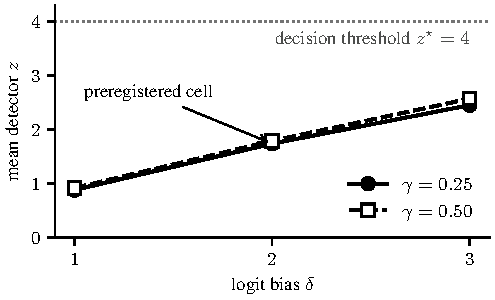
\includegraphics[width=\columnwidth]{figures/dose_response.pdf}
\caption{KGW dose response in the 7,200-generation calibration (10 keys, 40 tasks, 3 seeds per cell). Mean detector $z$ rises monotonically with bias $\delta$ at both greenlist ratios, but the preregistered cell stays well below the per-output threshold.}
\label{fig:dose}
\end{figure}

A first smoke run produced 960 generations with zero failures. All 480 watermarked outputs differed from their seeded baselines, so the processor was active. Mean $z$, however, was 0.995, and only 2/480 outputs reached $z\ge4$. An earlier run whose detector reconstructed the GPU-generated watermark on the CPU was archived as invalid, which is why the detector now runs on the same device as generation. The full calibration then varied $\gamma\in\{0.25,0.50\}$ and $\delta\in\{1,2,3\}$ over 10 keys, 40 tasks and 3 seeds, completing 7,200/7,200 generations. The primary cell was fixed in advance rather than chosen from these results.

Figure~\ref{fig:dose} shows a clean dose response: mean $z$ is 0.885/1.743/2.456 at $\gamma{=}0.25$ and 0.921/1.794/2.577 at $\gamma{=}0.50$ for $\delta=1/2/3$. This is evidence that the intervention is real and graded. At the primary cell, only 174/1200 outputs (14.5\%) reached $z\ge4$, far below the 80\% detection that Gate~N requires. Calibration took 1\,h\,59\,min to 2\,h\,17\,min per 720-generation job, or 9.9--11.4\,s per generation. This projects to roughly 200--230 L40S GPU-hours for the 72,720-generation main run.

\subsection{Ten-Key Security Pilot}
\begin{table}[t]
\centering
\small
\setlength{\tabcolsep}{3.2pt}
\begin{tabular}{@{}lrrrrrrr@{}}
\toprule
Key & Func. & S\&F & Sec$|$dec. & $\bot$ & Tok. & $\bar z$ & $z{\ge}4$ \\
\midrule
K0000 & 66.7 & 40.3 & 80.0 & 12 & 75.1 & $-0.21$ & 0 \\
K0001 & 12.5 & 5.6 & 80.0 & 12 & 77.7 & 0.56 & 0 \\
K0002 & 41.7 & 29.2 & 81.0 & 9 & 78.1 & $-1.09$ & 0 \\
K0003 & 37.5 & 20.8 & 79.7 & 13 & 78.8 & 1.44 & 0 \\
K0004 & 61.1 & 34.7 & 79.7 & 13 & 75.1 & 1.38 & 9 \\
K0005 & 65.3 & 38.9 & 79.7 & 13 & 74.9 & 0.62 & 0 \\
K0006 & 36.1 & 27.8 & 80.3 & 11 & 84.4 & $-0.10$ & 0 \\
K0007 & 62.5 & 37.5 & 80.0 & 12 & 84.0 & $-0.38$ & 0 \\
K0008 & \textbf{70.8} & \textbf{43.1} & 78.7 & 11 & 75.5 & 2.59 & 12 \\
K0009 & \underline{69.4} & \textbf{43.1} & 80.3 & 11 & 84.5 & $-0.13$ & 0 \\
\midrule
No WM & 58.3 & 36.1 & 79.7 & 13 & -- & -- & -- \\
\bottomrule
\end{tabular}
\caption{Security pilot: 24 tasks $\times$ 3 seeds $=$ 72 programs per arm, 792 in total, zero generation or scoring errors. Func.\ and S\&F are functional and secure-and-functional rates (\%); Sec$|$dec.\ is the secure share among decisively labelled outputs (\%); $\bot$ counts indeterminate security labels; Tok.\ is mean output length. Bold marks the highest and underline the second-highest watermarked rate. Because the keys are exploratory, these marks are descriptive and do not indicate a validated ``better'' key.}
\label{tab:pilot}
\end{table}

\begin{figure}[t]
\centering
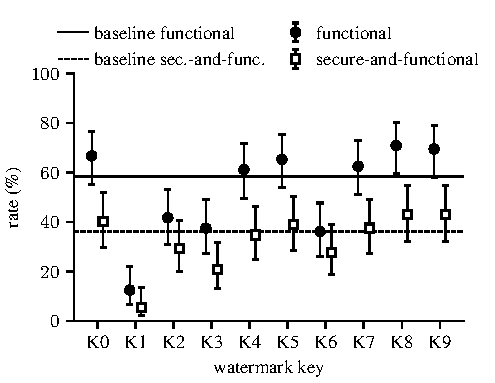
\includegraphics[width=\columnwidth]{figures/per_key_outcomes.pdf}
\caption{Per-key functional and secure-and-functional rates with row-level 95\% Wilson intervals; horizontal lines mark the shared unwatermarked baseline. The intervals ignore task clustering and are anti-conservative.}
\label{fig:perkey}
\end{figure}

Table~\ref{tab:pilot} and Figure~\ref{fig:perkey} summarise the pilot.

\textbf{Functional correctness varies widely across keys.} Functional rates range from 12.5\% (K0001, 9/72) to 70.8\% (K0008, 51/72), a spread of 58.3\,pp. The unwatermarked baseline is 58.3\%. The method-of-moments estimate attributes $\hat\sigma_\K\approx18.6$\,pp of across-key standard deviation to keys, against a mean within-key binomial standard error of 5.5\,pp. Because this naive estimate treats the 72 rows of a key as independent, it is only an illustration of the estimator. The secure-and-functional rate ranges from 5.6\% to 43.1\% (37.5\,pp; naive $\hat\sigma_\K\approx10.5$\,pp). The pooled watermarked rate, 231/720 (32.1\%), is not an inferential estimate of $\ATE$, because tasks and seeds repeat within it.

\textbf{Security labels are nearly key-invariant.} Every arm, including the baseline, has 12 or 13 secure-false labels. The secure share among decisive labels lies between 78.7\% and 81.0\% for every key. An inspection of labels by family found the path-traversal and XSS families uniformly insecure, the bounded-copy and bounded-format families almost uniformly indeterminate, and several Python families uniformly secure. Gate~O therefore fails, and almost all variation in $\Y$ is inherited from $\Fn$. A paired comparison illustrates how little the pilot can resolve: K0000 against its baseline gives 24 both-pass, 5 watermark-only, 2 baseline-only and 41 neither-pass cells. The exact McNemar test \citep{mcnemar1947note} gives $p=0.45$.

\subsection{Detector Diagnostics}
\begin{figure}[t]
\centering
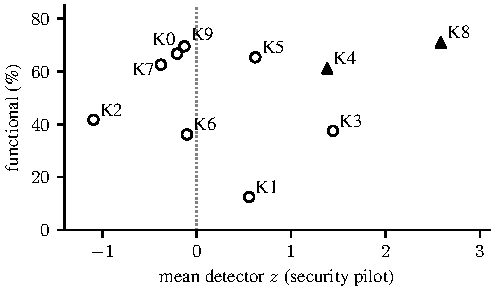
\includegraphics[width=\columnwidth]{figures/z_vs_functional.pdf}
\caption{Mean matching-key $z$ against functional rate per key. Triangles mark the two keys with any output at $z\ge4$. Five keys have a negative mean $z$, which a correctly aligned KGW processor should not produce on average.}
\label{fig:zfunc}
\end{figure}

Only 21/720 watermarked pilot outputs (2.9\%) reached $z\ge4$, and all of them came from K0004 (9) and K0008 (12). Pilot outputs averaged 75--85 tokens, compared with the longer calibration programs. Proposition~\ref{prop:length} predicts weak detection at this length: $T_{\min}=75$ tokens even at $p=0.45$, and the green fraction implied by K0008's mean $z$ is only about 0.38 (first-order estimate). Length does not explain the five keys with \emph{negative} mean $z$ (Figure~\ref{fig:zfunc}). Mean $z$ is also unrelated to functional rate across keys (Spearman $\rho=0.07$, $n=10$). So the functional spread is not simply ``stronger watermark, worse code''. Equally, until Gate~N passes, we cannot rule out that some keys were scored, or applied, differently from others.

\subsection{Threats to Validity}
\emph{Construct validity.} The security oracles in the pilot are saturated (Gate~O fails), so the pilot cannot measure a security effect in either direction. Static checks are not proof of security, which is why the next step integrates CWEval's outcome-driven tests unchanged \citep{peng2025cweval}. \emph{Internal validity.} The manipulation is unverified per key (Gate~N not yet run). The pilot configuration requested the model by branch name rather than commit hash; the validation and main-run configurations now pin a commit and pin PyTorch 2.6.0 and Transformers 5.22.2, but pilot rows predate that change. \emph{Statistical conclusion validity.} Ten keys and 24 tasks are too few to estimate $\sigma^2_\K$ reliably, and the intervals shown ignore clustering. \emph{External validity.} The study uses one model, one watermark family and two languages. The calibration used only the first 40 tasks of the controlled suite. \emph{Selection.} No key was selected on the outcomes reported here, and tail selection is reserved for discovery tasks.
